\documentclass[preview]{standalone}

\usepackage{amsmath}
\usepackage{amssymb}
\usepackage{tikz}
\usepackage{stellar}
\usepackage{definitions}
\usepackage{bettelini}

\begin{document}

\id{linearalgebra-cross-product}
\genpage

\section{Cross product}

\begin{snippetdefinition}{cross-product-definition}{Cross product}
    Let \(V\) be a real \vectorspace with \(\lineardim V=3\). Suppose that
    \(V\) is endowed with an \innerproduct and an \orientation. For
    \(u,v\in V\), the \emph{cross product} of \(u\) and \(v\), denoted
    \(u\times v\), is defined as follows.

    If \(u\) and \(v\) are linearly dependent, then
    \[
        u\times v=0.
    \]
    If \(u\) and \(v\) are \linearlyindependent, then \(u\times v\) is the
    unique vector of \(V\) such that:
    \begin{enumerate}
        \item \(u\times v\) is \orthogonal to both \(u\) and \(v\);
        \item \(\|u\times v\|\) is the area of the parallelogram generated
            by \(u\) and \(v\);
        \item \(\{u,v,u\times v\}\) is a positive ordered \basis of \(V\).
    \end{enumerate}
\end{snippetdefinition}

\begin{snippet}{cross-product-geometric-picture}
    Geometrically, \(u\times v\) is perpendicular to the plane generated by
    \(u\) and \(v\), its \norm is the area of the parallelogram generated by
    \(u\) and \(v\), and the \orientation chooses one of the two possible
    perpendicular directions.
    \[
        \begin{tikzpicture}[scale=0.9]
            \coordinate (O) at (0,0);
            \coordinate (U) at (3,0);
            \coordinate (V) at (1.1,1.7);
            \coordinate (S) at (4.1,1.7);

            \draw[->] (O) -- (U) node[right] {\(u\)};
            \draw[->] (O) -- (V) node[above left] {\(v\)};
            \draw[dashed] (U) -- (S);
            \draw[dashed] (V) -- (S);
            \draw[->] (O) -- (0,2.4) node[above] {\(u\times v\)};
            \node at (2.2,0.9) {area};
        \end{tikzpicture}
    \]
\end{snippet}

\begin{snippetproposition}{cross-product-existence-uniqueness}{Existence and uniqueness of the cross product}
    Let \(V\) be a real \vectorspace with \(\lineardim V=3\), endowed with
    an \innerproduct and an \orientation. If \(u,v\in V\) are
    \linearlyindependent, then there exists a unique vector \(u\times v\)
    satisfying the three conditions in the definition of the \crossproduct.
\end{snippetproposition}

\begin{snippetproof}{cross-product-existence-uniqueness-proof}{cross-product-existence-uniqueness}{Existence and uniqueness of the cross product}
    Since \(u\) and \(v\) are \linearlyindependent,
    \(\linearspan(u,v)\) has dimension \(2\). Its orthogonal complement has
    dimension \(1\). Hence there are exactly two unit vectors orthogonal to
    both \(u\) and \(v\), namely \(w\) and \(-w\). The \orientation selects
    the one for which \(\{u,v,w\}\) is a positive ordered \basis.

    If \(\alpha\) is the angle between \(u\) and \(v\), the parallelogram
    generated by \(u\) and \(v\) has area
    \[
        \|u\|\,\|v\|\sin\alpha.
    \]
    Therefore
    \[
        u\times v=\|u\|\,\|v\|\sin\alpha\, w
    \]
    is forced, and it satisfies the defining conditions.
\end{snippetproof}

\begin{snippet}{cross-product-area-picture}
    If \(\alpha\) is the angle between \(u\) and \(v\), the height of the
    parallelogram over the side \(u\) is \(\|v\|\sin\alpha\). Thus its area
    is \(\|u\|\,\|v\|\sin\alpha\).
    \[
        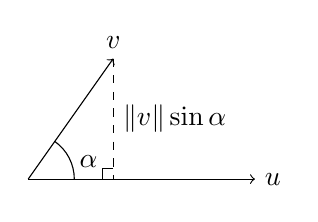
\begin{tikzpicture}[scale=0.9]
            \coordinate (O) at (0,0);
            \coordinate (U) at (3.2,0);
            \coordinate (V) at (1.2,1.7);
            \coordinate (P) at (1.2,0);

            \draw[->] (O) -- (U) node[right] {\(u\)};
            \draw[->] (O) -- (V) node[above] {\(v\)};
            \draw[dashed] (V) -- (P);
            \draw (1.05,0) -- (1.05,0.15) -- (1.2,0.15);
            \draw (0.65,0) arc (0:55:0.65);
            \node at (0.85,0.25) {\(\alpha\)};
            \node[right] at (1.2,0.85) {\(\|v\|\sin\alpha\)};
        \end{tikzpicture}
    \]
\end{snippet}

\section{Properties}

\begin{snippetproposition}{cross-product-basic-properties}{Basic properties of the cross product}
    Let \(V\) be a real \vectorspace with \(\lineardim V=3\), endowed with
    an \innerproduct and an \orientation. For every \(u,v\in V\),
    \begin{enumerate}
        \item \(u\times v=-v\times u\);
        \item \(u\times v=0\) if and only if \(u\) and \(v\) are linearly
            dependent;
        \item the map
            \[
                V\cartesianprod V\fromto V,
                \qquad
                (u,v)\mapsto u\times v
            \]
            is bilinear.
    \end{enumerate}
\end{snippetproposition}

\begin{snippetproof}{cross-product-basic-properties-proof}{cross-product-basic-properties}{Basic properties of the cross product}
    The second property is part of the definition when \(u\) and \(v\) are
    linearly dependent. If they are \linearlyindependent, the parallelogram
    has positive area, so \(u\times v\neq 0\).

    For the first property, assume \(u\) and \(v\) are
    \linearlyindependent. The vectors \(u\times v\) and \(v\times u\) have
    the same \norm and are both orthogonal to \(\linearspan(u,v)\). Swapping
    the order of \(u\) and \(v\) reverses the \orientation of the ordered
    basis, so \(v\times u=-(u\times v)\). If \(u\) and \(v\) are dependent,
    both sides are zero.

    For bilinearity, choose a positive \orthonormalbasis
    \[
        \{e_1,e_2,e_3\}
    \]
    of \(V\). In this basis,
    \[
        e_1\times e_2=e_3,
        \qquad
        e_2\times e_3=e_1,
        \qquad
        e_3\times e_1=e_2,
    \]
    and the remaining products follow by anti-commutativity and
    \(e_i\times e_i=0\). Expanding vectors in this basis gives a bilinear
    formula, hence the \crossproduct is bilinear.
\end{snippetproof}

\begin{snippetexample}{cross-product-positive-orthonormal-basis-formula}{Formula in a positive orthonormal basis}
    Let \(V\) be a real oriented \(3\)-dimensional \innerproductspace, and
    let
    \[
        \{e_1,e_2,e_3\}
    \]
    be a positive \orthonormalbasis of \(V\). If
    \[
        u=u_1e_1+u_2e_2+u_3e_3,
        \qquad
        v=v_1e_1+v_2e_2+v_3e_3,
    \]
    then
    \[
        u\times v
        =
        e_1(u_2v_3-u_3v_2)
        -
        e_2(u_1v_3-u_3v_1)
        +
        e_3(u_1v_2-u_2v_1).
    \]
    Equivalently,
    \[
        u\times v
        =
        \begin{vmatrix}
            e_1 & e_2 & e_3\\
            u_1 & u_2 & u_3\\
            v_1 & v_2 & v_3
        \end{vmatrix}.
    \]
\end{snippetexample}

\begin{snippetcorollary}{r3-cross-product-formula}{Cross product in R3}
    In \(\realnumbers^3\) with the canonical \innerproduct and canonical
    \orientation, if
    \[
        u=(u_1,u_2,u_3),
        \qquad
        v=(v_1,v_2,v_3),
    \]
    then
    \[
        u\times v
        =
        (u_2v_3-u_3v_2,\,
        u_3v_1-u_1v_3,\,
        u_1v_2-u_2v_1).
    \]
\end{snippetcorollary}

\end{document}
